\documentclass[../piano-di-qualifica.tex]{subfiles}


\begin{document}
\subsection{Analisi statica dei documenti}%
\label{sub:analisi_statica_doc}
Per l'analisi statica dei documenti GruppOne ha utilizzato il package \glossario{chktex} che ha consentito di trovare errori nella sintassi latex.
Il test, eseguito automaticamente, impedisce l'approvazione definitiva se vengono segnalati errori.

\begin{figure}[H]
  \centering
  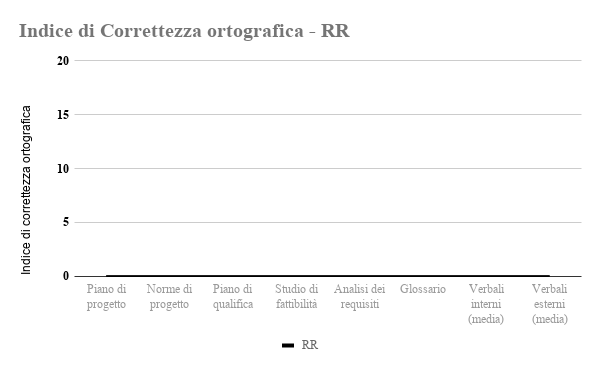
\includegraphics[width=160mm]{correttezzaortografica-RR.png}%
  \caption{Indice di correttezza ortografica \- RR}%
  \label{fig:indice_correttezza_ortografica_RR}%
\end{figure}


\begin{figure}[H]
  \centering
  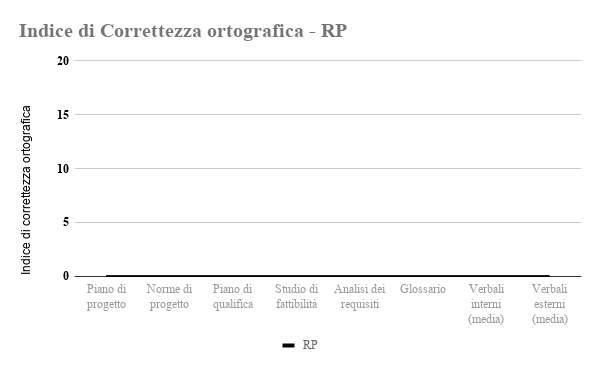
\includegraphics[width=160mm]{correttezzaortografica-RP.png}%
  \caption{Indice di correttezza ortografica \- RP}%
  \label{fig:indice_correttezza_ortografica_RP}%
\end{figure}



% sub:analisi_statica_doc (end)
\subsection{Esito verifica leggibilità}%
\label{sub:verifica_leggibilita}
Allo scopo di assicurarci una leggibilità accettabile dei documenti abbiamo monitorato l'indice \glossario{Gulpease} di ogni documento. Qui sotto riportiamo i risultati associati alle versioni consegnate in occasione delle revisioni di avanzamento relativamente agli obiettivi di qualità che erano stati definiti.
\rowcolors{2}{lightgray}{white!80!lightgray!100}
\begin{longtable}[H]{>{\centering\bfseries}m{6cm} >{\centering\arraybackslash}m{2cm} >{\centering\arraybackslash}m{2cm}>{\centering\arraybackslash}m{2cm} >{\centering\arraybackslash}m{4cm}}
  \rowcolor{darkgray!90!}
  \color{white}{\textbf{Documento}} & \color{white}{\textbf{RR}} & \color{white}{\textbf{RP}} & \color{white}{\textbf{Esito dell'ultima verifica}} \\
  Piano di Progetto                 & 96                         & 95                         & Sufficiente                                        \\
  Norme di Progetto                 & 68                         & 74                         & Sufficiente                                        \\
  Piano di Qualifica                & 81                         & 83                         & Sufficiente                                        \\
  Studio di Fattibilità             & 65                         & ---                        & Sufficiente                                        \\
  Analisi dei requisiti             & 100                        & 100                        & Sufficiente                                        \\
  Glossario                         & 74                         & 83                         & Sufficiente                                        \\
  Verbali esterni (media)           & 77                         & 74                         & Sufficiente                                        \\
  Verbali interni (media)           & 80                         & 77                         & Sufficiente                                        \\
  \rowcolor{white}
  \caption{Attualizzazione dei rischi per la fase di incremento 1}%
  \label{tab:attualizzazione_per_la_fase_di_incremento_1}
\end{longtable}
% \begin{figure}[H]
%   \centering
%   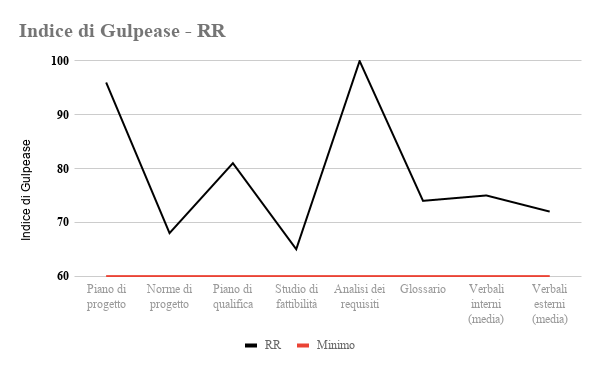
\includegraphics[width=160mm]{gulpease-RR.png}%
% \end{figure}

% \begin{figure}[H]
%   \centering
%   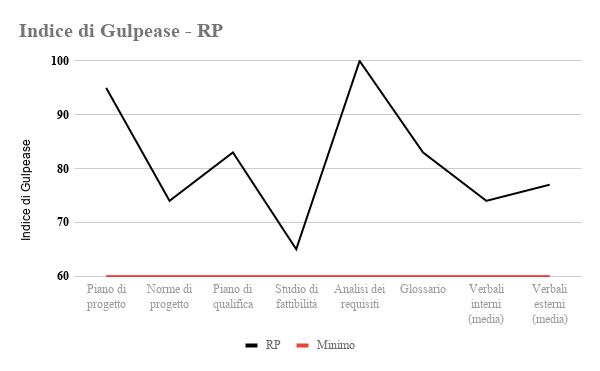
\includegraphics[width=160mm]{gulpease-RP.png}%
% \end{figure}


\begin{figure}[H]
  \centering
  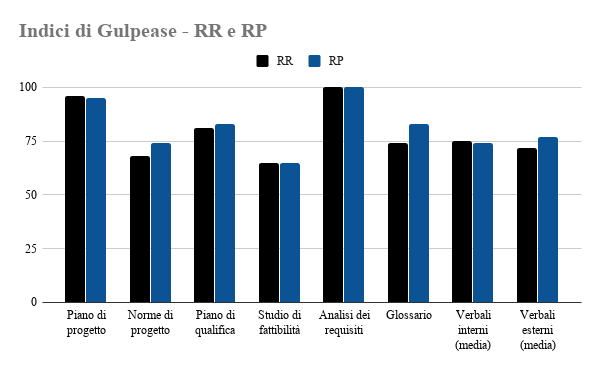
\includegraphics[width=160mm]{gulpease-conf.png}%
  \caption{Indice di Gulpease}%
  \label{fig:gulpease}%
\end{figure}

\newpage

\subsection{Qualità di sviluppo}%
\label{sub:analisi_statica_doc}
Per la qualità di sviluppo del software GruppOne ha utilizzato \glossario{SonarCloud} che permette di eseguire diverse tipologie di test black-box.


\begin{figure}[H]
  \centering
  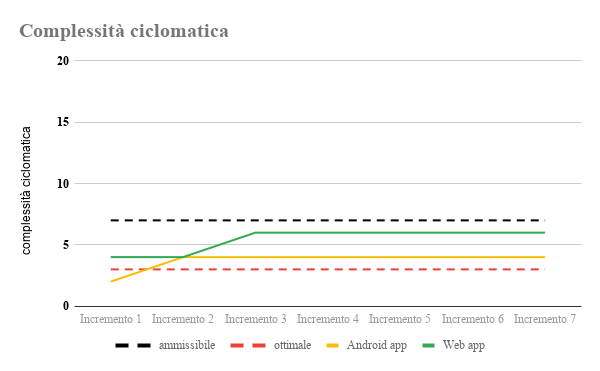
\includegraphics[width=160mm]{compl_ciclomatica.png}%
  \caption{Complessità ciclomatica}%
  \label{fig:compl_ciclomatica}%
\end{figure}


\begin{figure}[H]
  \centering
  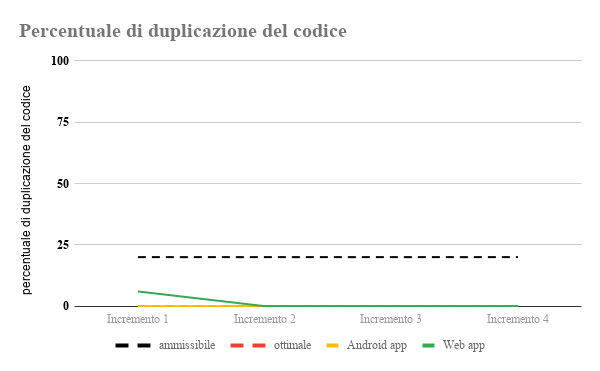
\includegraphics[width=160mm]{duplicazione_codice.png}%
  \caption{Duplicazione codice}%
  \label{fig:duplicazione_codice}%
\end{figure}

\begin{figure}[H]
  \centering
  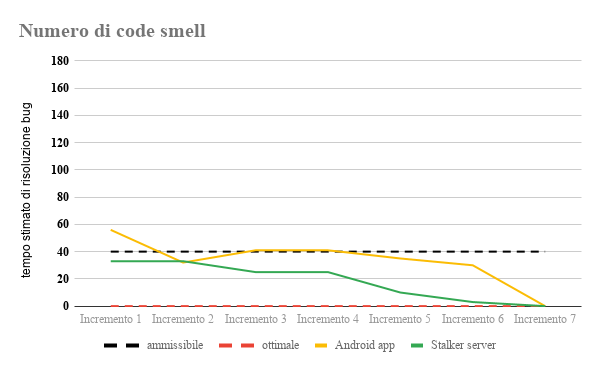
\includegraphics[width=160mm]{code_smell.png}%
  \caption{Code smell}%
  \label{fig:code_smell}%
\end{figure}


\begin{figure}[H]
  \centering
  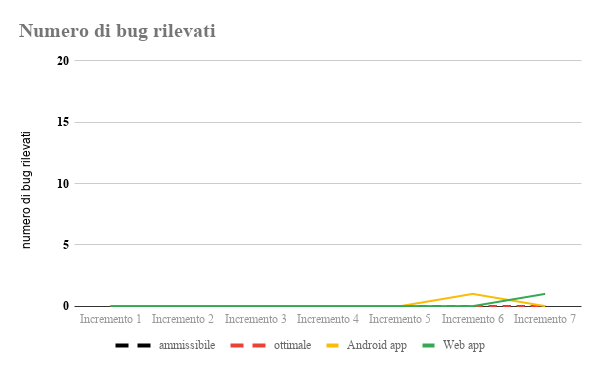
\includegraphics[width=160mm]{bug_rilevati.png}%
  \caption{Bug rilevati}%
  \label{fig:bug_rilevati}%
\end{figure}

\begin{figure}[H]
  \centering
  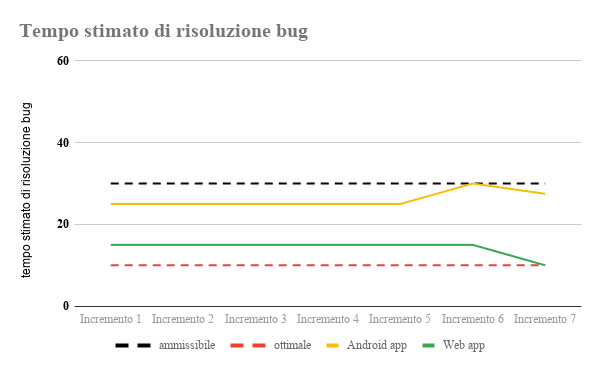
\includegraphics[width=160mm]{tempo_stimato_bug.png}%
  \caption{Tempo stimato bug}%
  \label{fig:tempo_stimato_bug}%
\end{figure}


\newpage

\subsection{Discostamenti orari ed economici}%
\label{sub:discostamenti_orari_ed_economici}
Per assicurarci di rispettare il preventivo, abbiamo monitorato i discostamenti, in percentuale, fra il lavoro eseguito e quello pianificato, dai punti di vista economico ed orario. Nel seguito riportiamo i risultati al termine di ogni fase.

\begin{figure}[H]
  \centering
  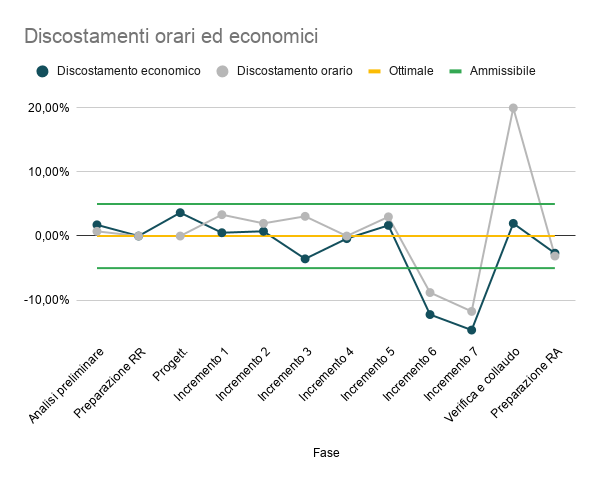
\includegraphics[width=160mm]{discostamenti-orari-economici.png}%
  \caption{Discostamenti orari ed economici}%
  \label{fig:discostamenti_orari_economici}%
\end{figure}
% sub:discostamenti_orari_ed_economici (end)

\subsection{Metriche con valore ottimale}%
\label{sub:metriche_ottimali}
Infine, alla fine di ogni fase misuriamo quante metriche raggiungono valori definiti come ottimali per avere una visione complessiva dell'andamento della qualità nei controlli.
\begin{figure}[H]
  \centering
  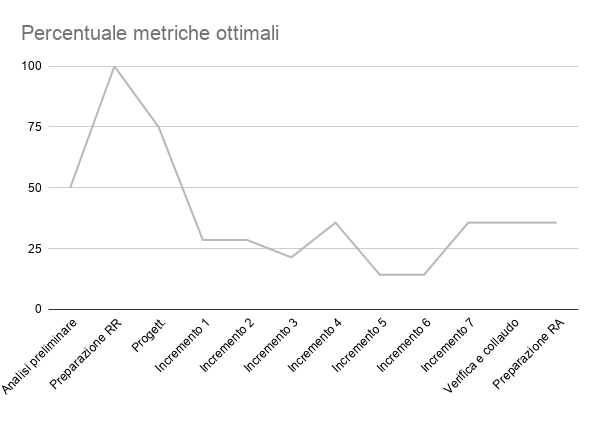
\includegraphics[width=160mm]{percentualemetricheottimali.png}%
  \caption{Percentuale di metriche ottimali}%
  \label{fig:metriche_ottimali}%
\end{figure}
% sub:metriche_ottimali (end)

\end{document}
